\chapter{Introduction}


For robots to make a smooth ingress into dynamic human environments like home and office, the robots need to be able to close the \emph{perceive-action-learning} loop. Essentially these domestic service robots should perceive the environment, interact with the environment, learn from experiences and repeat. The robot interacts with the environment by choosing a sequence of low-level actions . For example, lets take the high-level task of ``making tea", this will require the following actions to be executed sequentially: fill the kettle, boil water, find the teabag, find a cup, put teabag into the cup and pour hot water into the cup. But for executing some of the actions like finding the kettle, finding teabag, finding cup etc. requires the robot to have prior knowledge about the possible locations. Such knowledge about the environment or the user needs to be learned by the robot. The goal of this thesis is to enable domestic service robots to gain knowledge about common behaviours and preferences of the user in a non-intrusive manner. Specifically, we address how Bayesian methods can be used to provide a flexible and computationally efficient structure for acquiring knowledge using limited spatio-temporal information collected by these service robots.

Domestic service robots need to have the ability to automatically and quickly adapt to a new environment. Imagine if the robot could learn how the user arranges the breakfast table by looking at the data from previous days. Robots can observe the users lifestyle and provide small insights which the user doesn't even notice. The robots can pass along helpful information to the users, like observing their sleep habits and tell them when they are not having adequate sleeps. By learning how the user interacts with their homes and how they live their lives, robots will be able to provide better services to their users. 


\begin{figure}[htp]
\centering
\begin{subfigure}{\textwidth}
  \centering
  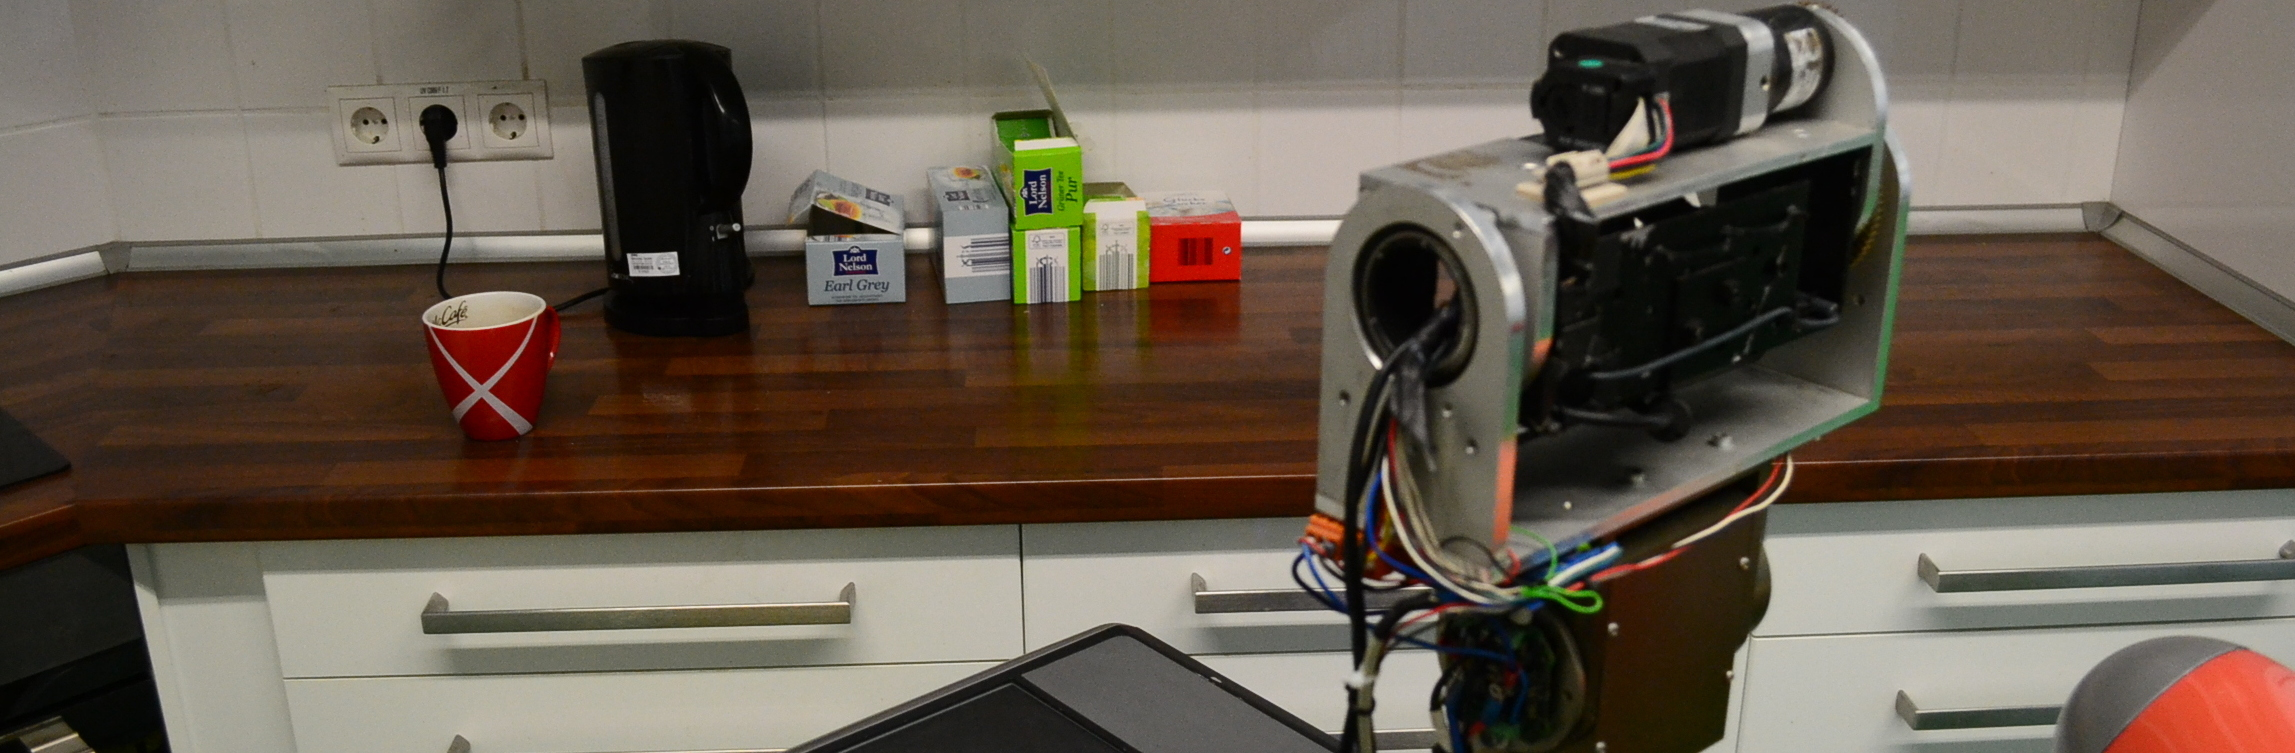
\includegraphics[width=\linewidth]{images/introduction.jpg}
\end{subfigure}%
\\
\begin{subfigure}{.24\textwidth}
  \centering
  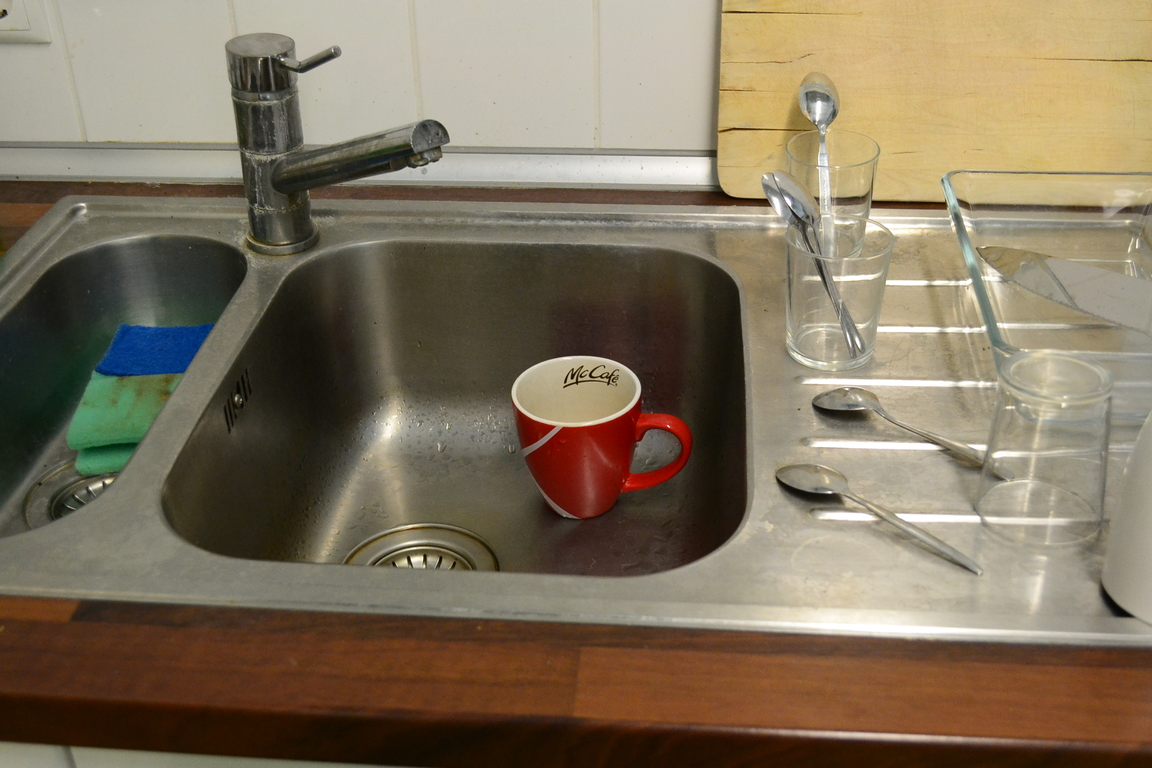
\includegraphics[width=\linewidth]{images/cup_sink.jpg}
  \caption{cup in sink}
\end{subfigure}
\begin{subfigure}{.24\textwidth}
  \centering
  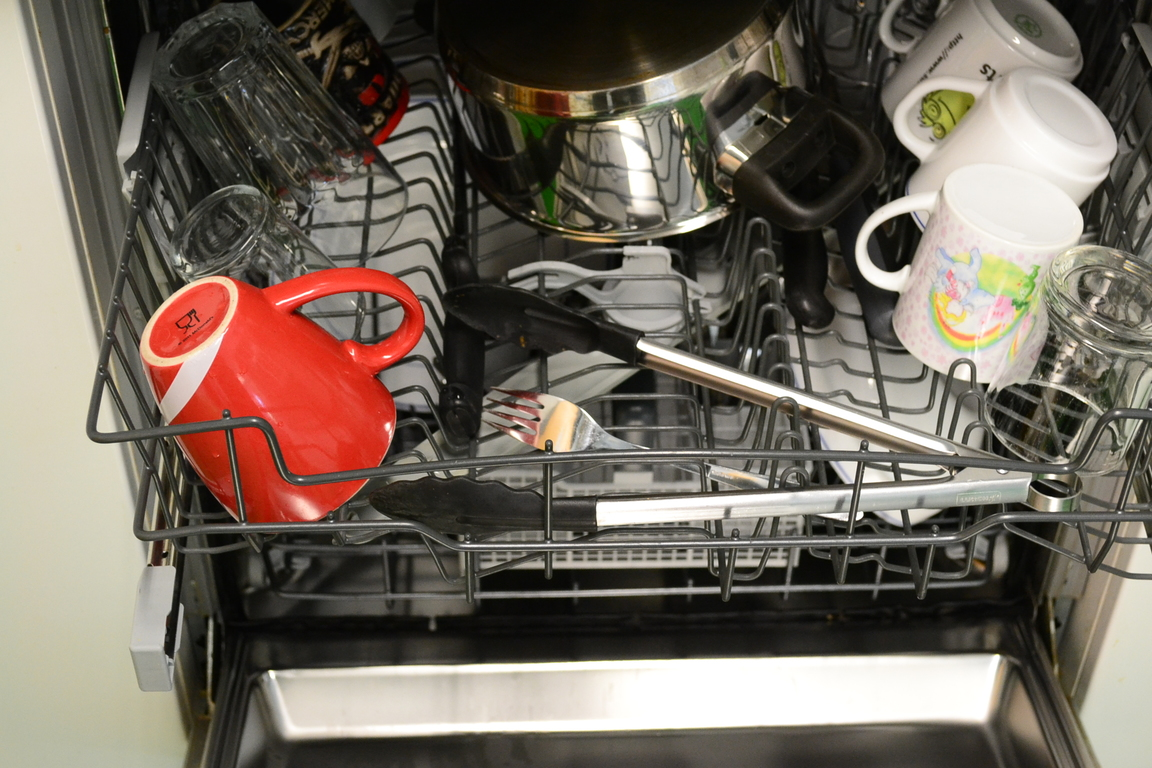
\includegraphics[width=\linewidth]{images/cup_dishwasher.jpg}
    \caption{cup in dishwasher}
\end{subfigure}
\begin{subfigure}{.24\textwidth}
  \centering
  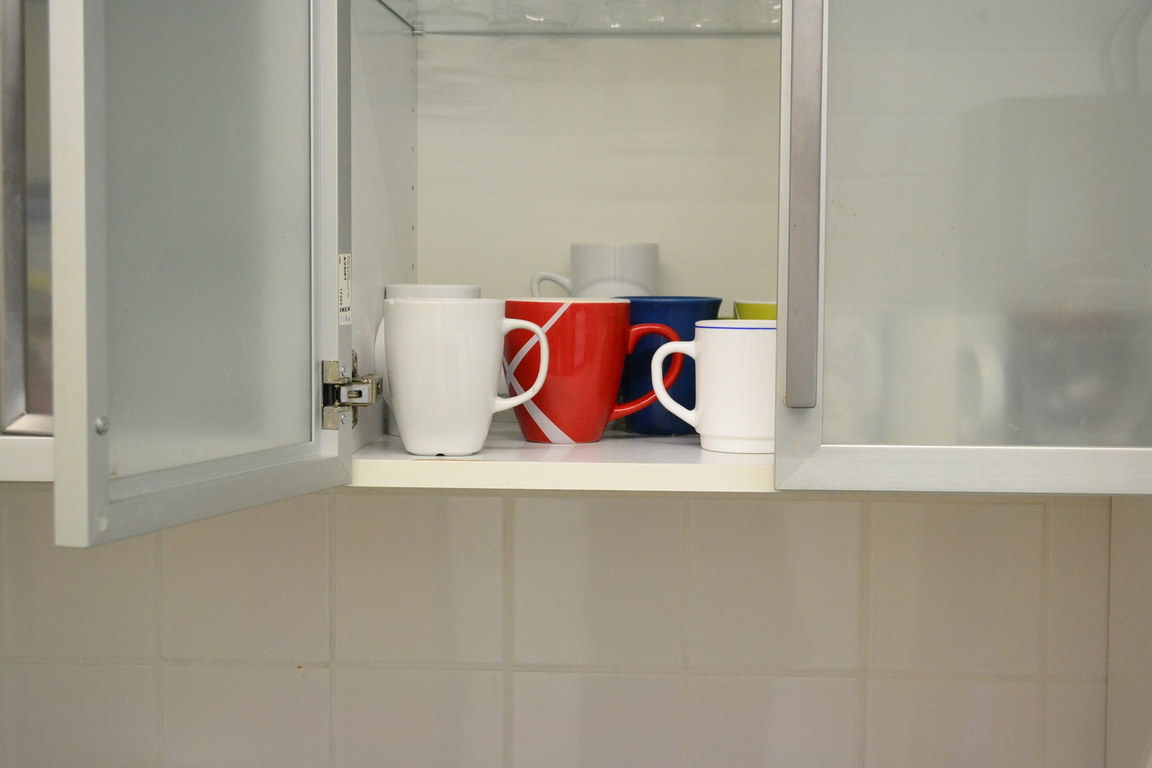
\includegraphics[width=\linewidth]{images/cup_cupboard.jpg}
    \caption{cup in cupboard}
\end{subfigure}
\begin{subfigure}{.255\textwidth}
  \centering
  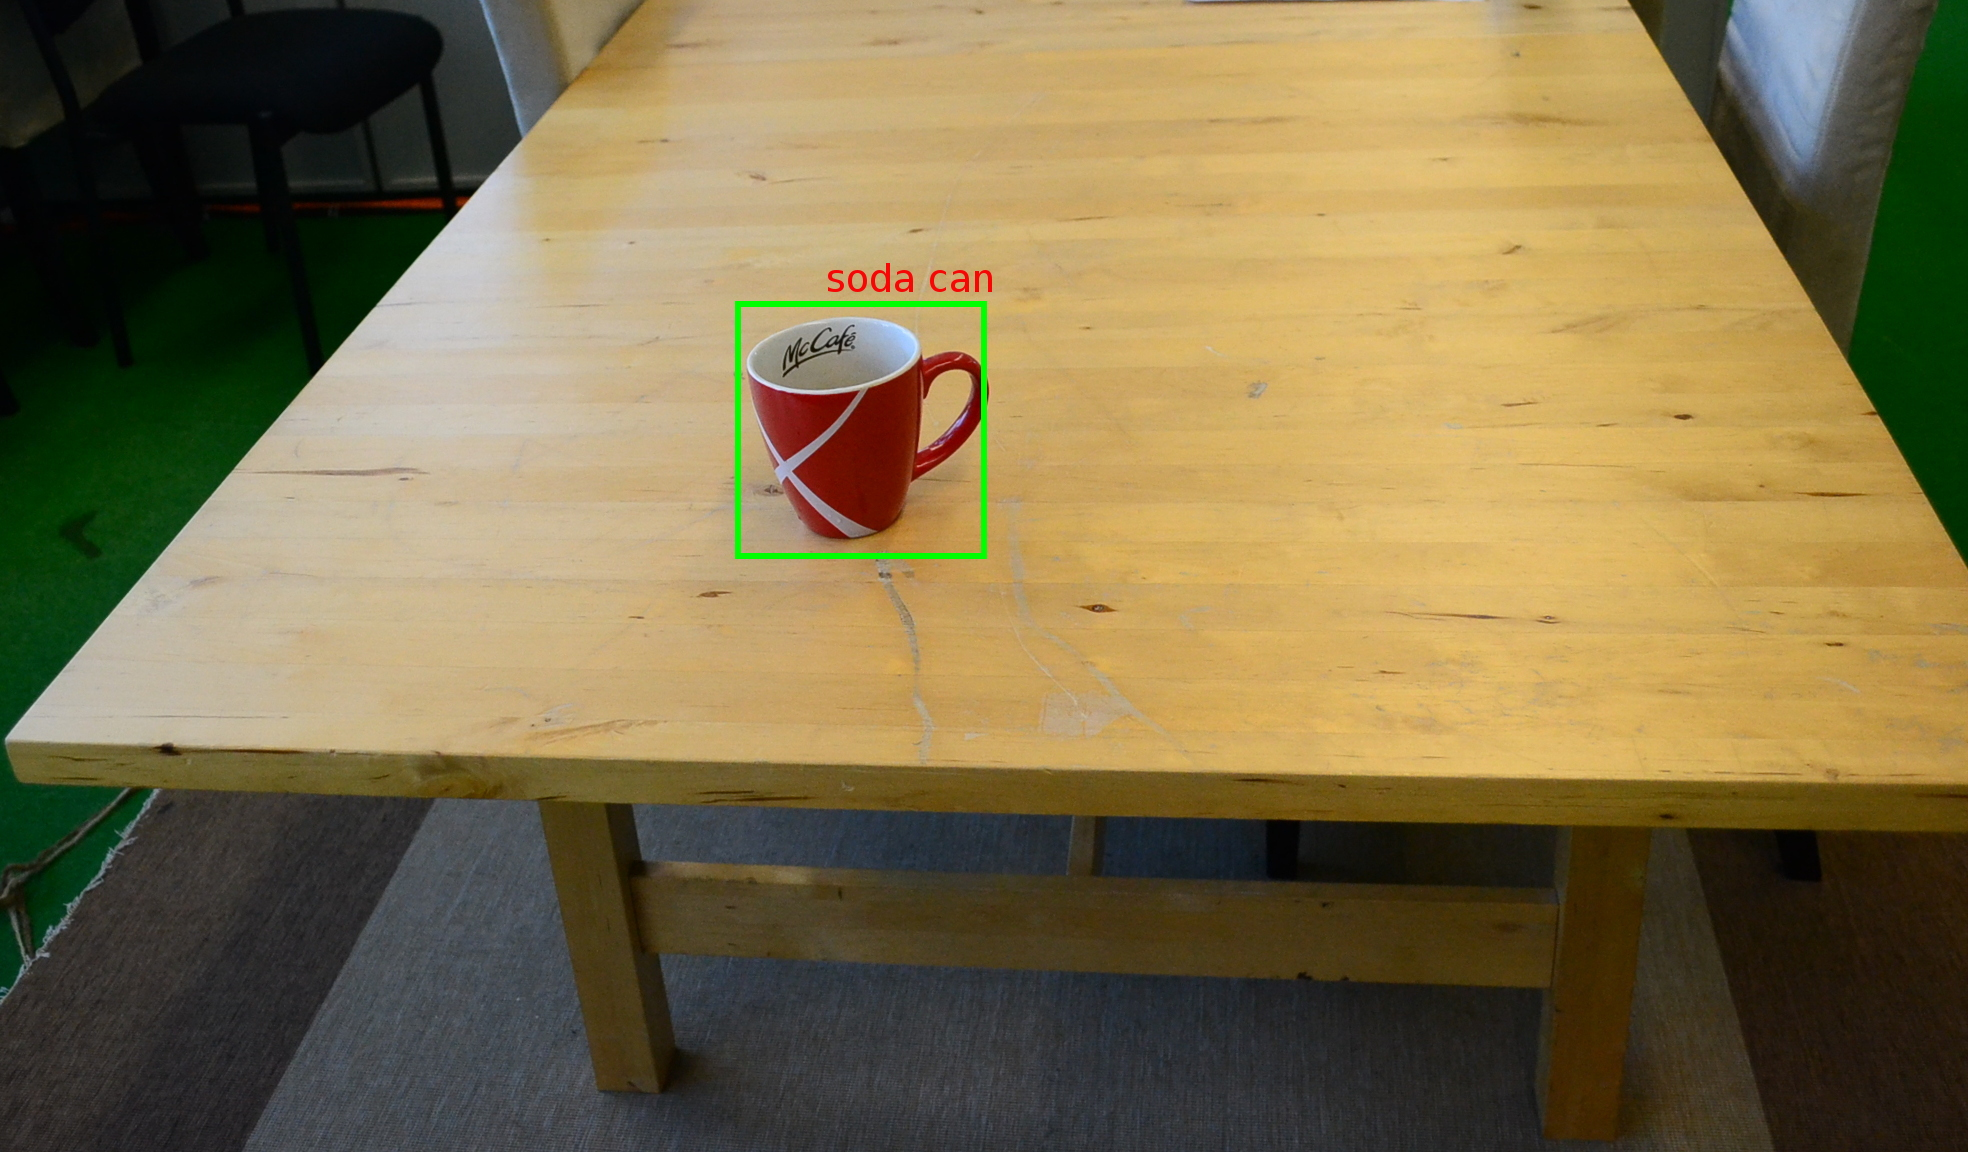
\includegraphics[width=\linewidth]{images/robot_view_cup.jpg}
    \caption{cup on table}
\end{subfigure}

\caption[Illustrative example]{Illustrative example of the robot making a record of all the information it has generated in its memory for learning user preferences in object placements}
\end{figure}

Domestic service robots while interacting with the user and environment produce information which after being processed in perception, actuation, or decision making are discarded. \cite{niemueller2012generic} has proposed an approach of storing these information in a robot memory and produce useful knowledge. 
The domestic robot will continuously record sightings of objects and persons with position and time in a database to form the spatio-temporal robot memory. Machine learning is the best method for automatic knowledge generation from the stored information. But in order to adapt quickly the robot needs to able to extract valuable knowledge from small amount of information, i.e., the learning algorithms need to be data efficient.

To illustrate the relevance of the topics presented in this thesis, we motivate our work using a typical task of a domestic service robot.   We assume that the robot is given the task of ``making coffee" for the user, which requires the robot to locate the coffee cup of the user first, make coffee and then to locate the user, for delivering the coffee to him. To begin the search for the coffee cup, it would help the robot to have some prior knowledge about the user's habits; in particular the typical locations where he keeps his cup. This enables the robot to funnel its search for the object from a large number of locations to the most probable ones. Once the coffee cup is located and grasped the robot needs to reason about where it can currently find the user for delivering it to him. This in turn, requires the robot to have knowledge about the likely locations of Waldo at that time.

This motivating example leads us to the two research topics in knowledge acquisition we address in this thesis:
\begin{enumerate}
	\item How can a domestic service robot acquire knowledge about user preferences in placing objects in the environment?
	\item How can a domestic service robot acquire knowledge about the user's temporal location behaviour?
	\item How can a domestic service robot acquire the above knowledge using small amounts of information?
\end{enumerate}

A service robot operating in dynamic human environments needs to perceive the world using its own sensors, and subsequently build a cognitive model of the user preferences and behaviour. These models represent the internal beliefs of the robot about the user preferences and behaviour. The model needs to be extract the knowledge from small amount of information, basically we should develop methods to do data-efficient machine learning. There are many approaches that demonstrate that data-efficient machine learning is possible, including methods like: explicit domain knowledge modelling, exploiting structural knowledge of data, bootstrapping and data augmentation, semi-supervised learning, transfer learning, active learning and Bayesian optimization, non-parametric methods, one-shot learning and Bayesian deep learning \cite{https://sites.google.com/site/dataefficientml/home}. 
Bayesian probabilistic formulation of the cognitive model makes it possible to include the above mentioned methods in a single framework. The robots can use these models to predict the future behaviour of the user or can make educated guess about the user while doing actions with partial information.


In sum, this thesis provides Bayesian probabilistic techniques that enable a domestic service robot
\begin{itemize}
	\item to learn the user preference model in object placement.
	\item to learn the user's temporal location behaviour model.
	\item to learn in the absence of information.
\end{itemize}

\todo[inline]{TODO: add chapter flow}

All of our approaches are based on state-of-the art Bayesian learning techniques such as Dirichlet processes, graphical models and probabilistic programming. The probabilistic formulation of our approaches allows the robot to represent the state of its knowledge or the state of its belief. In an exhaustive set of experiments on real-world and simulated datasets we show that our approaches are able to successfully extract knowledge about user behaviours and preferences from observations made by a domestic service robot. Furthermore, we also demonstrate that the acquired knowledge can be utilized in smart decision making frameworks which can accommodate vision recognition faults. We hope that our approaches will set up service robots into the existing household by knowing what and who are there and adapting to them. These service robots will grow and change with the users, with a greater awareness of the world around them

